% Author: Victor Terron (c) 2013
% Email: `echo vt2rron1iaa32s | tr 132 @.e`
% License: CC BY-SA 4.0

\documentclass[14pt]{beamer}

\usepackage[utf8]{inputenc}
\usepackage{listings}
\usepackage[T1]{fontenc}

% A Nice Title Page for Beamer Presentations
% http://github.com/dfalster/BeamerTitleSlide
\usepackage{tikz}
\usepackage[framemethod=tikz]{mdframed}

% Define a new mdframed environment
\newmdenv[tikzsetting={draw=black,fill=white,fill opacity=0.65},
  backgroundcolor=none,leftmargin=0,rightmargin=0, innertopmargin=4pt,
  skipbelow=\baselineskip, skipabove=\baselineskip]{TitleBox}

% Reduce space between image and caption; also remove prefix 'Figure:'
% http://tex.stackexchange.com/a/94018
% http://tex.stackexchange.com/a/82462
\usepackage[font=small,skip=1pt,labelformat=empty]{caption}

% New line between paragraphs, no indentation
% http://tex.stackexchange.com/q/42
\usepackage[parfill]{parskip}

\usetheme{Copenhagen}
\useoutertheme{infolines}
\setbeamercovered{dynamic}
\setbeamertemplate{navigation symbols}{} % remove navigation symbols

\lstset{basicstyle=\ttfamily,language=python}

% Remove the space symbol for code inside the double quotation marks
% http://www.latex-community.org/viewtopic.php?f=4&t=248
\lstset{showstringspaces=false}

% Enable accents and ñ in our code listings
% http://stackoverflow.com/a/2782147/184363
\lstset{
  literate={á}{{\'a}}1
           {é}{{\'e}}1
           {í}{{\'i}}1
           {ó}{{\'o}}1
           {ú}{{\'u}}1
           {ñ}{{\~n}}1
           {¡}{{\textexclamdown}}1
}

% \input a file in the ./puntos/ directory
\newcommand{\punto}[1]{\input{./puntos/#1}}

\definecolor{red}{HTML}{F41B1B}
\definecolor{darkerred}{HTML}{DE2931}
\definecolor{blue}{HTML}{2E3CEC}
\definecolor{green}{HTML}{3C8031}

% Beamer: footer with current slide number but not total slide number
% http://tex.stackexchange.com/a/32815
\makeatletter
\setbeamertemplate{footline}
{
  \leavevmode%
  \hbox{%
  \begin{beamercolorbox}[wd=.333333\paperwidth,ht=2.25ex,dp=1ex,center]{author in head/foot}%
    \usebeamerfont{author in head/foot}\insertshortauthor~~\beamer@ifempty{\insertshortinstitute}{}{(\insertshortinstitute)}
  \end{beamercolorbox}%
  \begin{beamercolorbox}[wd=.333333\paperwidth,ht=2.25ex,dp=1ex,center]{title in head/foot}%
    \usebeamerfont{title in head/foot}\insertshorttitle
  \end{beamercolorbox}%
  \begin{beamercolorbox}[wd=.333333\paperwidth,ht=2.25ex,dp=1ex,right]{date in head/foot}%
    \usebeamerfont{date in head/foot}\insertshortdate{}\hspace*{2em}
    \insertframenumber\hspace*{2ex}
  \end{beamercolorbox}}%
  \vskip0pt%
}
\makeatother

\title{["Python"] * 40}
\author{Víctor Terrón}
\date{23 de noviembre de 2013}
\institute{IAA-CSIC}

\begin{document}

\section{Introducción}

\begin{frame}
  \titlepage

  \begin{figure}
    \vspace{-0.5cm}
    
\includegraphics[width=2cm]{pics/mistery-box.jpg}
  \end{figure}

  \footnotesize
  \begin{center}
    Cuarenta características de Python que \structure{quizás} no conoces
  \end{center}

\end{frame}

% Author: Victor Terron (c) 2014
% Email: `echo vt2rron1iaa32s | tr 132 @.e`
% License: CC BY-SA 4.0

\begin{frame}{Programación orientada a objetos}
  \small
  \begin{block}
    {\centering Una cita apócrifa}
    \centering
    ``Object-oriented programming is an exceptionally bad
    idea which could only have originated in California''
    [Edsger W. Dijkstra]
  \end{block}

  \begin{figure}
    \centering
    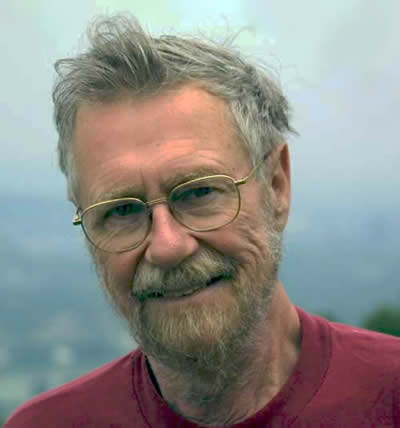
\includegraphics[height=4cm]{pics/dijkstra.jpg}
  \end{figure}
\end{frame}

\begin{frame}{Programación orientada a objetos}
  \small
  \begin{block}
    {\centering Lo que en realidad dijo}
    \centering
    ``For those who have wondered: I don't think object-oriented
    programming is a structuring paradigm that meets my standards of
    elegance.'' [Edsger W. Dijkstra, 1999]
    [\href{http://www.cs.utexas.edu/users/EWD/transcriptions/EWD12xx/EWD1284.html}
      {\structure{Fuente}}]
  \end{block}

  \begin{figure}
    \centering
    
\includegraphics[height=5cm]{pics/like-a-sir.png}
  \end{figure}
\end{frame}

\begin{frame}{Programando clases en Python}
  \begin{block}{}
    \Large
    \centering
    El objetivo de esta charla es ayudarnos a hacer
    \structure{idiomáticas} y \structure{elegantes} nuestras clases en
    Python.
  \end{block}

  \begin{justify}
    En mayor o menor medida todo el mundo usa programación orientada a
    objetos, pero hay una serie de aspectos fundamentales que es
    indispensable conocer para evitar que nuestro código sea
    innecesariamente feo o complejo.
  \end{justify}
\end{frame}

\begin{frame}{Nuestra reacción a veces}
  \begin{figure}
    \centering
    
\includegraphics[height=6cm]{pics/dont-want-to-live-on-this-planet.png}
  \end{figure}
\end{frame}

\begin{frame}{Programando clases en Python}
  \begin{alertblock}{}
    \small
    \centering
    La premisa es que somos mínimamente familiares con los
    \structure{conceptos básicos} de programación orientada a objetos,
    y que hemos trabajado un poco con nuestras propias clases en
    Python.
  \end{alertblock}

  \begin{figure}
    \centering
    
\includegraphics[height=4cm]{pics/captain-obvious.jpg}
  \end{figure}
\end{frame}

\begin{frame}{Un muy brevísimo repaso}
  \begin{itemize}
    \item Llamamos \structure{clase} a la representación abstracta de un
      concepto. Por ejemplo, 'perro', 'número entero' o 'servidor web'.
    \item Las clases se componen de \structure{atributos} y
      \structure{métodos}.
    \item Un objeto es cada una de las instancias de una clase.
  \end{itemize}
\end{frame}

\begin{frame}{Ejemplo: clase Perro}
  \pythoncode[fontsize=\footnotesize]{intro.py}
\end{frame}

\begin{frame}{¡No os limitéis a escuchar!}
  \begin{center}
    No suele ser divertido escuchar a nadie hablar durante casi una
    hora. Participad, intervenid, criticad, opinad. ¡Si digo algo que
    no tiene ningún sentido, \structure{corregidme}!
  \end{center}

  \begin{block}{\centering El código fuente está disponible en:}
    \centering \url{http://github.com/vterron/PyConES-2014}
  \end{block}

  \begin{center}
    \small Erratas, correcciones, enlaces, ¡cualquier cosa!
  \end{center}
\end{frame}


\begin{frame}{}
  \begin{alertblock}{}
    \centering \Large ¿Listos?
  \end{alertblock}

  \begin{figure}
    \centering
    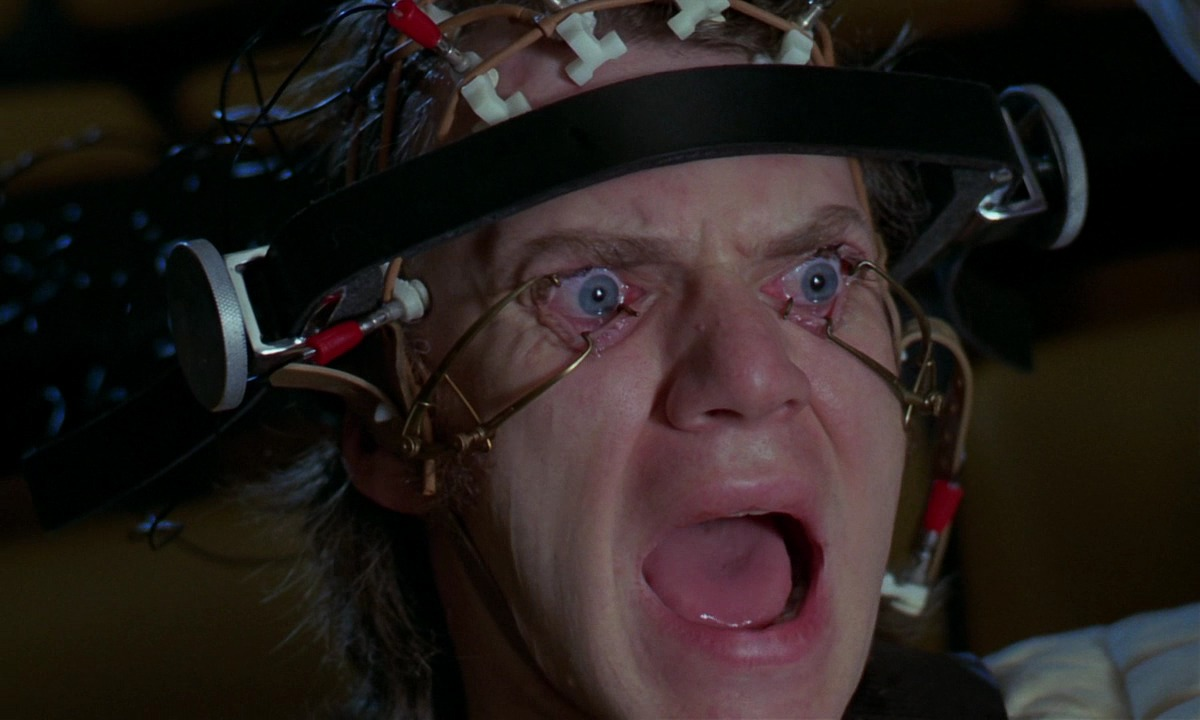
\includegraphics[height=6cm]{pics/a-clockwork-orange.jpg}
  \end{figure}
\end{frame}

\section{Los diez primeros}

\punto{01.tex}
\punto{02.tex}
\punto{03.tex}
\punto{04.tex}
\punto{05.tex}
\punto{06.tex}
\punto{07.tex}
\punto{08.tex}
\punto{09.tex}
\punto{10.tex}

\section{Los diez siguientes}

\punto{11.tex}
\punto{12.tex}
\punto{13.tex}
\punto{14.tex}
\punto{15.tex}
\punto{16.tex}
\punto{17.tex}
\punto{18.tex}
\punto{19.tex}
\punto{20.tex}

\section{}

\begin{frame}{}
  \begin{block}{}
    \centering \Large Respira profundamente
  \end{block}

  \begin{figure}
    \centering
    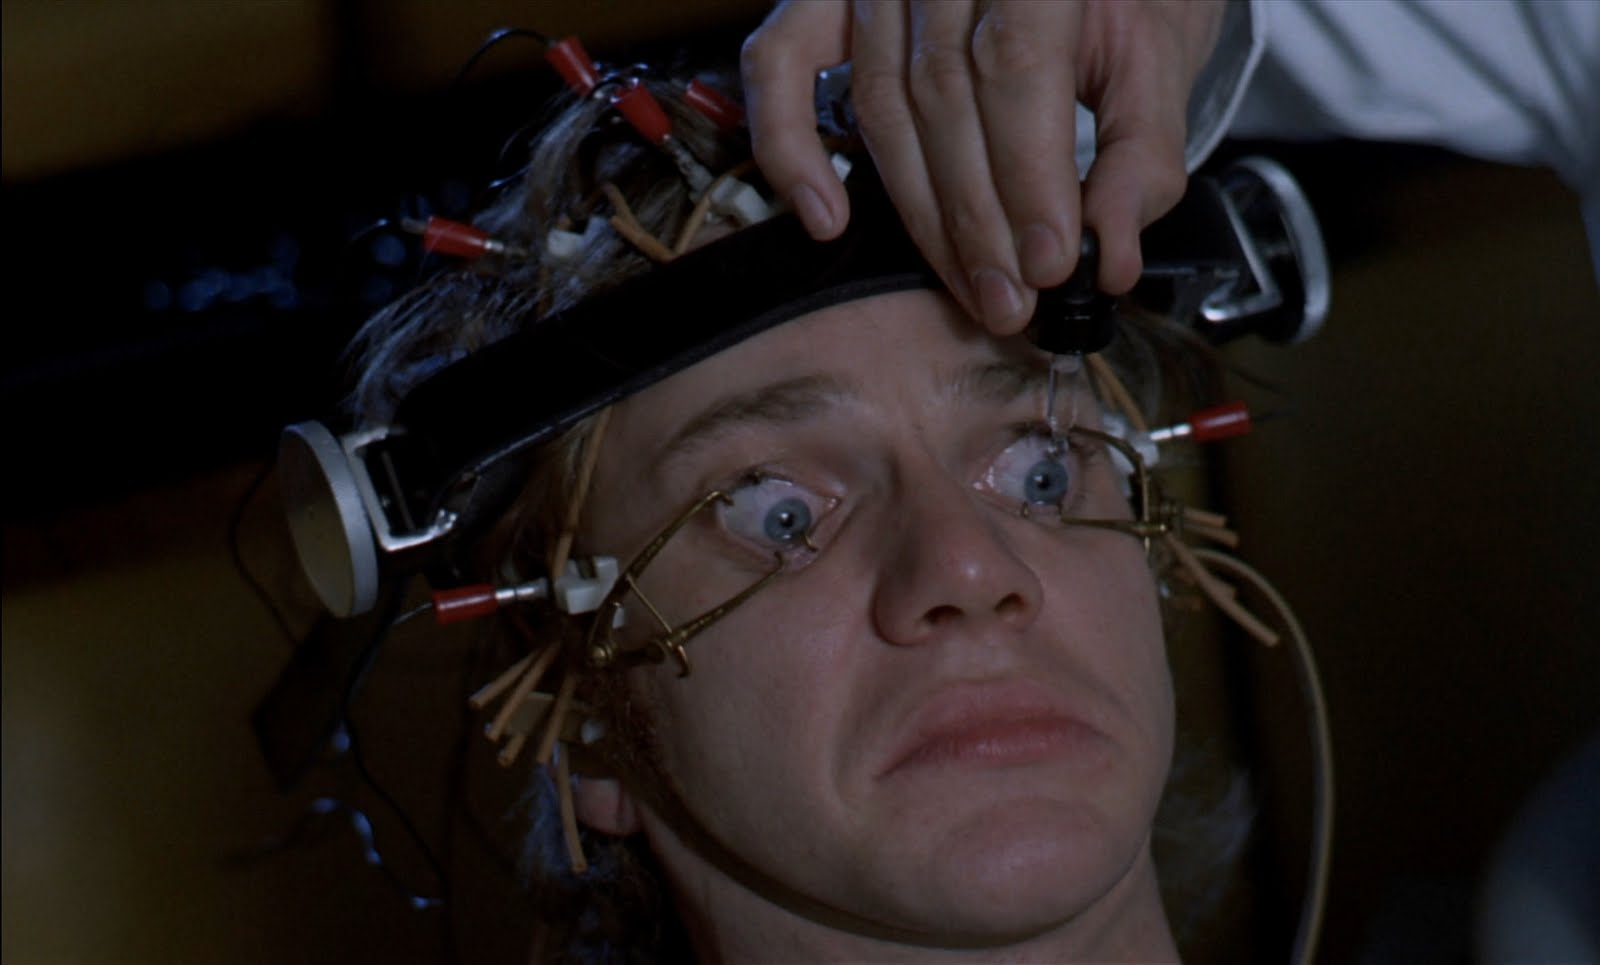
\includegraphics[height=6cm]{pics/a-clockwork-orange-2.jpg}
  \end{figure}
\end{frame}

\section{Diez más}

\punto{21.tex}
\punto{22.tex}
\punto{23.tex}
\punto{24.tex}
\punto{25.tex}
\punto{26.tex}
\punto{27.tex}
\punto{28.tex}
\punto{29.tex}
\punto{30.tex}

\section{Recordatorio}
\begin{frame}[fragile]{A veces nos sentimos así}
  \begin{figure}
    \centering
    
\includegraphics[height=0.75\paperheight]{pics/first-day-internet.jpg}
  \end{figure}
\end{frame}

\section{Los últimos diez}

\punto{31.tex}
\punto{32.tex}
\punto{33.tex}
\punto{34.tex}
\punto{35.tex}
\punto{36.tex}
\punto{37.tex}
\punto{38.tex}
\punto{39.tex}
\punto{40.tex}

\section{You Are Now a Ninja}
\begin{frame}{Programadores Python Shaolín}
  \begin{figure}
    \centering
    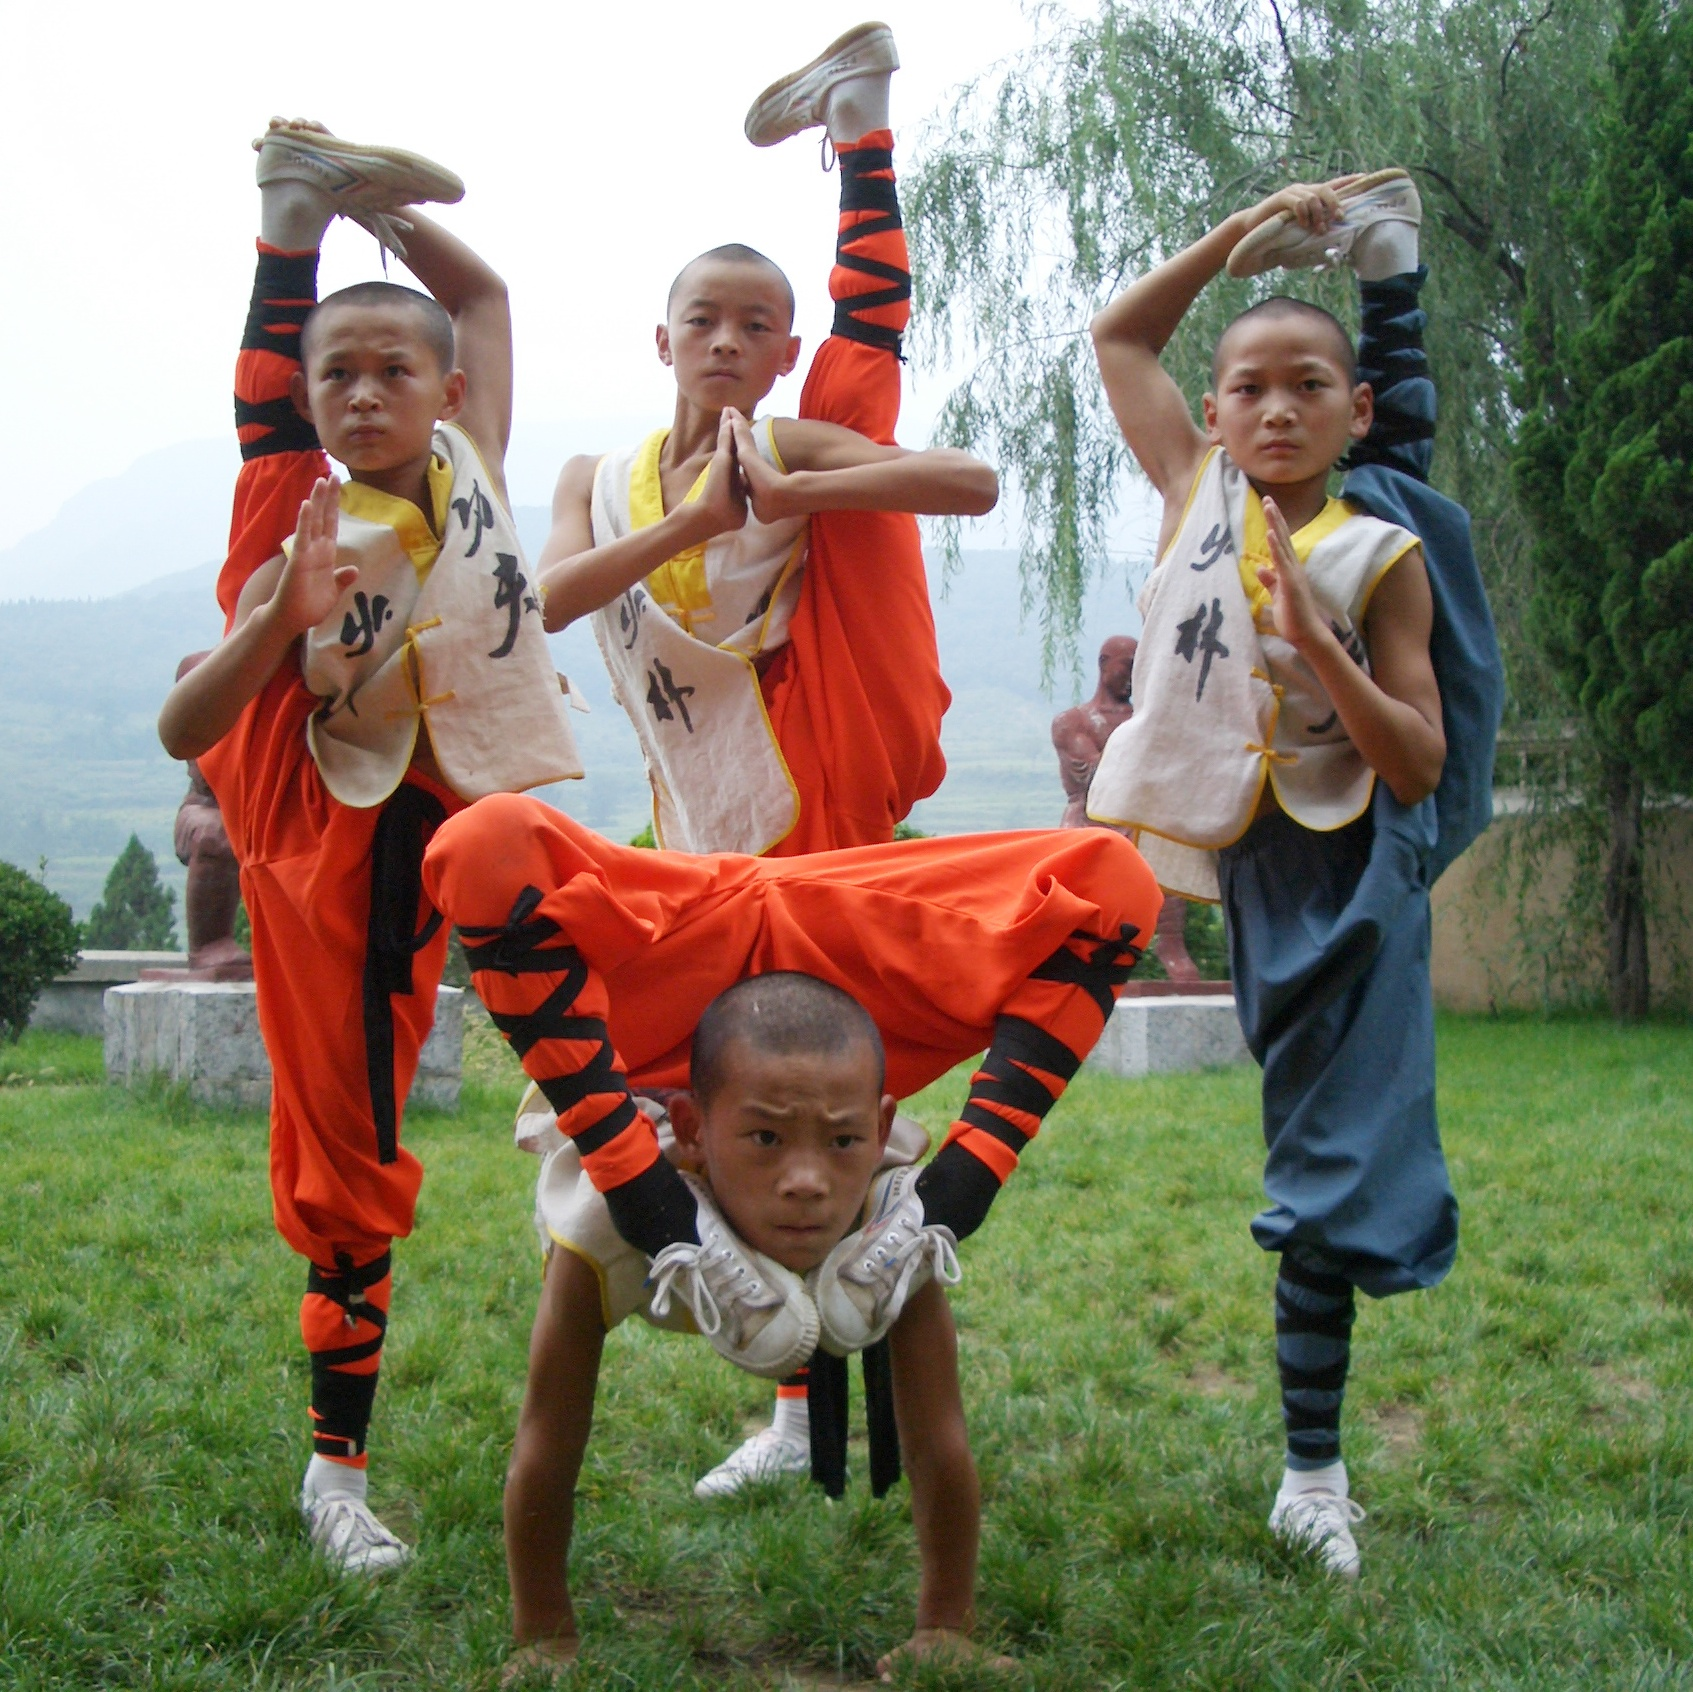
\includegraphics[height=7cm]{pics/shaolin.jpg}
  \end{figure}
\end{frame}

\end{document}
